\documentclass[12pt,letterpaper,twoside]{article}

\newif\ifsolution\solutiontrue   % Include the solutions
%\newif\ifsolution\solutionfalse  % Exclude the solutions

\usepackage{cme213}
\usepackage{xcolor}
\usepackage{graphicx}

\newcommand{\T}[1]{\text{\texttt{#1}}}
\newcommand{\V}[1]{\text{\textit{#1}}}

\begin{document}

{\centering \textbf{Homework 3\\ Due Sunday, May 1st via GradeScope\\}}
\vspace*{-8pt}\noindent\rule{\linewidth}{1pt}

\paragraph{Problem 1: Recurrence } Implement a simple CUDA program for 
a recurrence relation (inspired by the Mandelbrot Set) for many 
different starting points.

\begin{itemize}
    \item \textbf{1.1 Allocate GPU memory} Idea: Use \texttt{cudaMalloc}
    to allocate memory on the GPU device for both the input and output 
    arrays we will need for the recurrence implementation. Free memory 
    with \texttt{cudaFree} at end of \texttt{main()}.

\begin{cpp}
// Allocate num_bytes of memory to the device arrays
cudaMalloc(&device_input_array, num_bytes);
cudaMalloc(&device_output_array, num_bytes);
...
...

// Deallocate memory from both device arrays
cudaFree(device_input_array);
cudaFree(device_output_array);
\end{cpp}

    \item \textbf{1.2 Initialize array of random floats} Idea: Use in-built
    rand() functor from the standard cpp library and scale it between -1 
    and 1 as required.

\begin{cpp}
// Initialize an array of size arr_size in input_array with 
//random floats between -1 and 1
void initialize_array(vec &input_array, size_t arr_size) {
    input_array.resize(arr_size);
    std::generate(input_array.begin(), input_array.end(), rand);

    for(int i=0; i<arr_size; i++){
    input_array[i] = static_cast<float>(input_array[i])/
                        (RAND_MAX/2)-1;
    }    
}
\end{cpp}

    \item \textbf{1.3 Implement recurrence kernel} Idea: Recurrence operations 
    themselves are not independent and therefore not parallelizable, however, 
    we can parallelize doing many of these recurrence loops for different 
    starting points (constants). So, we want to parallelize over our 1-dim 
    input array of constants.

    Since our kernel needs to handle cases where the number of threads is less 
    than the number of entries in our input array, we need to use a grid-stride 
    loop.

\begin{cpp}
/**
* Implement the kernel recurrence.
* The CPU implementation is in host_recurrence() in main_q1.cu.
*/
__global__ void recurrence(const elem_type* input_array,
                            elem_type* output_array, 
                            size_t num_iter,
                            size_t array_length) {

    for (int xid = blockIdx.x * blockDim.x + threadIdx.x;
        xid < array_length;
        xid += blockDim.x * gridDim.x) {
    
        elem_type z = 0;
        elem_type constant = input_array[xid];

        int it=0;
        while(it<num_iter) {
        z = z * z + constant;
        it++;
        }
        output_array[xid] = z;
    }
}
\end{cpp}
    
    Console logs.
\begin{verbatim}
Starting at Fri Apr 29 00:28:45 UTC 2022

nvcc -O3 -std=c++11 -arch=compute_75 -code=sm_75 -o main_q1 main_q1.cu

Output from main_q1
----------------
Largest error found at pos: 15 error 7.81565e-08 
    expected 1.52526 and got 1.52526

Largest error found at pos: 0 error 0 
    expected 0.680375 and got 0.680375

Largest error found at pos: 439038 error 1.19193e-07 
    expected 1.00014 and got 1.00014

Largest error found at pos: 142710 error 2.38333e-07 
    expected 2.00072 and got 2.00072

Largest error found at pos: 482709 error 5.61004e-07 
    expected 16.9994 and got 16.9994

Largest error found at pos: 482709 error 1.15797e-06 
    expected 289.897 and got 289.898

Largest error found at pos: 482709 error 2.324e-06 
    expected 84041.4 and got 84041.6

Largest error found at pos: 482709 error 4.63941e-06 
    expected 7.06296e+09 and got 7.063e+09

Largest error found at pos: 482709 error 9.25711e-06 
    expected 4.98854e+19 and got 4.98859e+19

Largest error found at pos: 138972 error 1.79297e-05 
    expected 8.03779e+21 and got 8.03765e+21

Largest error found at pos: 905817 error 2.59306e-05 
    expected 1.66519e+35 and got 1.66523e+35

Questions 1.1-1.3: your code passed all the tests!
\end{verbatim}

    \item \textbf{1.4 Vary number of threads per block} When we 
    vary number of threads per block while holding number of 
    iterations (40,000), array size (1e6) and grid size (72) 
    constant, we get the plot shown below. 
    
    \begin{figure}[h]
        \center
        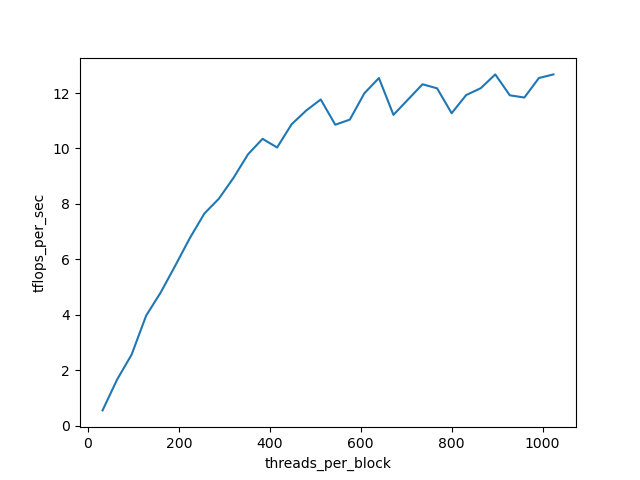
\includegraphics[scale=0.7]{q1_4.png}
        \caption{Performance as we vary number of threads per block}
    \end{figure}

    Performance improves roughly linearly with threads per block 
    for the first ~400 threads, after which we get asymptotic 
    behaviour and a saw-tooth pattern. This is because we reach 
    the point where the overhead incurred from additional threads
    starts to dominate performance benefit of computing incremental 
    recurrence relations in parallel.

    \item \textbf{1.5 Vary number of blocks} When we 
    vary number of blocks (grid size) while holding number of 
    iterations (40,000), array size (1e6) and threads per block 
    (128) constant, we get the plot shown below. 

    \begin{figure}[h]
        \center
        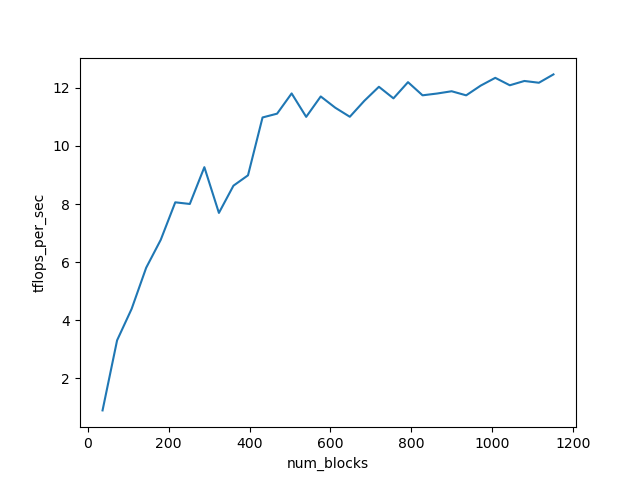
\includegraphics[scale=0.7]{q1_5.png}
        \caption{Performance as we vary number of blocks}
    \end{figure}

    Performance improves roughly linearly with number of blocks 
    for the first ~200 blocks, after which we get asymptotic 
    behaviour and a saw-tooth pattern. Similar to q1.4, this is 
    because we reach the point where the overhead incurred from 
    additional blocks starts to dominate performance benefit of 
    computing incremental recurrence relations in parallel.

    \item \textbf{1.6 Vary number of iterations} When we 
    vary number of iterations while holding number of threads 
    per block (256), number of blocks (576) and array size (1e6) 
    constant, we get the plot shown below. 
    
    \begin{figure}[h]
        \center
        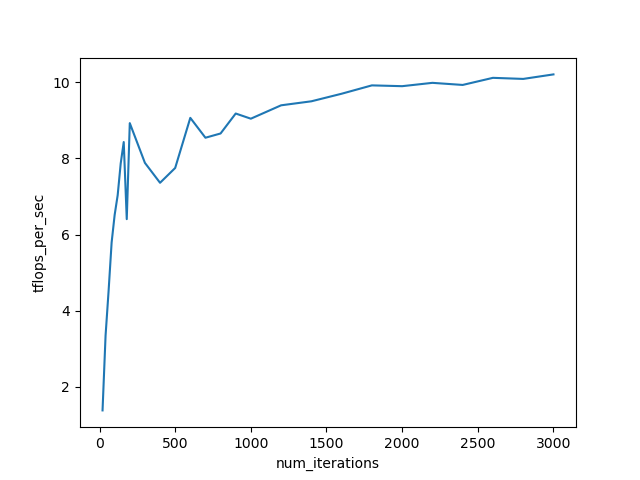
\includegraphics[scale=0.7]{q1_6.png}
        \caption{Performance as we vary number of iterations}
    \end{figure}

    Performance jumps quickly to ~7 Tflops per second as we increase
    number of iterations from 20-120, after which we get asymptotic 
    behaviour and a saw-tooth pattern. Iteratiions are done sequentially
    and so a higher number of iterations means that each thread takes 
    longer to complete its task before reassigned. This initially means
    that we reduce overhead of assigning threads per iterations, but 
    eventually we are working with tasks that are too big to spread
    evenly across threads (i.e. last thread running has a large portion
    of its task still to complete).
    
\end{itemize}


\paragraph{Problem 2: PageRank} Implement a simplified PageRank link analysis
algorithm that generates a score for every node in a graph by considering 
links to adjacent nodes.

\begin{itemize}
    \item \textbf{2.1: Implement PageRank algorithm} Idea: Want to parallelize
    update of each node across gpu threads since independent. Since recurrence 
    relationship itself must be serial, we will need to sync our threads after 
    each complete update. We do this by relaunching the kernel for each 
    iteration step.

    Code snippet for kernel.
\begin{cpp}
/* 
* Each kernel handles the update of one pagerank score. In other
* words, each kernel handles one row of the update:
*
*      pi(t+1) = A pi(t) + (1 / (2N))
*/
__global__ void device_graph_propagate(
    const uint *graph_indices,
    const uint *graph_edges,
    const float *graph_nodes_in,
    float *graph_nodes_out,
    const float *inv_edges_per_node,
    int num_nodes
) {
    for (int i = blockIdx.x * blockDim.x + threadIdx.x;
        i < num_nodes;
    i += blockDim.x * gridDim.x) 
    {
        float sum = 0.f;    

        for (int j = graph_indices[i]; j < graph_indices[i+1]; j++) 
        {
        sum += graph_nodes_in[graph_edges[j]] * 
            inv_edges_per_node[graph_edges[j]];
        }
        graph_nodes_out[i] = 0.5f / (float)num_nodes + 0.5f * sum;
    }
}
\end{cpp}

    \item \textbf{2.2: Compute bandwidth by hand} Idea: Figure out by hand the number 
    of bytes read from and written to global memory by the algorithm.

    For each iteration, for each node,
    \begin{itemize}
        \item Read ints \texttt{graph\_indices[i]} and \texttt{graph\_indices[i+1]} 
        \item Read int \texttt{graph\_edges[j]} * average number of edges
        \item Read float \texttt{graph\_nodes\_in[]} * average number of edges
        \item Read float \texttt{inv\_edges\_per\_node[]} * average number of edges
        \item Write float \texttt{graph\_nodes\_out[i]}
    \end{itemize}
    Sub-total = sizeof(int) * (2 + edges) + sizeof(float) * (1 + 2 * edges)

    Total = sub-total * nodes * iterations

\begin{cpp}
/**
* This function computes the number of bytes read from and written to
* global memory by the pagerank algorithm.
* 
* nodes: the number of nodes in the graph
* edges: the average number of edges in the graph
* iterations: the number of iterations the pagerank algorithm was run
*/
uint get_total_bytes(uint nodes, uint edges, uint iterations)
{
    int subtotal = sizeof(int)*(2+1*edges) + sizeof(float)*(1+2*edges);
    return iterations * nodes * subtotal;
}
\end{cpp}

    \item \textbf{2.3: Plot bandwidth vs number of nodes} Plot device
    memory bandwidth in Gb/sec as we increase number of nodes, while holding
    average number of edges constant.

    \begin{figure}[h]
        \center
        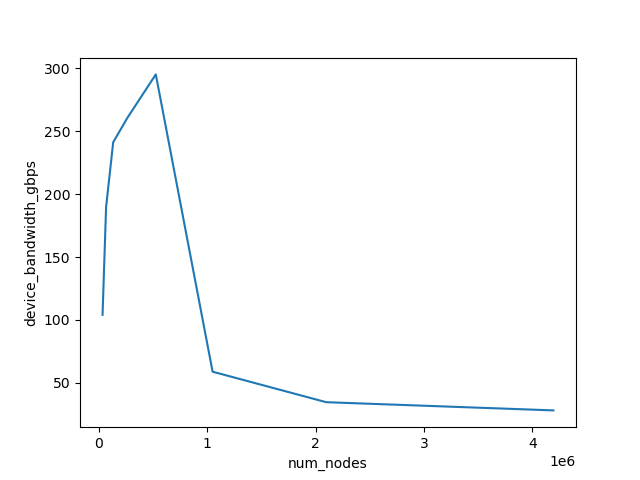
\includegraphics[scale=0.7]{q2_2.png}
        \caption{Device bandwidth as we increase number of nodes}
    \end{figure}

    \item \textbf{2.4: Comment on memory bandwidth plot} Our device bandwidth 
    reaches an optimal of ~300 Gb/sec near 500,000 nodes, with performance 
    dropping sharply either side. This is the point where our memory access
    is most aligned and coalesced!
    
    What does the memory access pattern look like? Our PageRank program has 
    a mix of sequential and random access patterns. For each node, it fetches
    2 contiguous ints that specifies the relevant range of indices in our 
    edge array, which we need access sequentially to find each adjacent node.
    However, the adjacent nodes themselves are not necessarily stored 
    contiguously in memory within the input and inverse degree arrays, 
    and so accessing these for each edge is roughly random access.

    Explain the differnce between Problem 2 and maximum bandwidth of 480 GB/sec? 
    Achieving maximum bandwidth performance would require that our memory access
    completely aligned and coalesced. We would need our access pattern to 
    be completely sequential to maximize prefetching.

\end{itemize}


\paragraph{Problem 3: Strided Memory Access} Benchmark our device by performing
strided memory access in \texttt{benchmark.cu}.


\begin{itemize}
    \item \textbf{3.1: Benchmark strided access} ...

    \item \textbf{3.2: Comment on shape of graph} ...

    Why do we observe the trend that we do as the stride length increases?

\end{itemize}


Submission information logs.
\begin{verbatim}
jelc@cardinal1:~$ /afs/ir.stanford.edu/class/cme213/script/submit.py hw2 private/cme213-jelc53/hw2
Submission for assignment 'hw2' as user 'jelc'
Attempt 1/10
Time stamp: 2022-04-13 20:09
List of files being copied:
    private/cme213-jelc53/hw2/sum.h	 [768 bytes]
    private/cme213-jelc53/hw2/parallel_radix_sort.h	 [7625 bytes]

Your files were copied successfully.
Directory where files were copied: /afs/ir.stanford.edu/class/cme213/submissions/hw2/jelc/1
List of files in this directory:
    sum.h	 [768 bytes]
    parallel_radix_sort.h	 [7625 bytes]
    metadata	 [137 bytes]

This completes the submission process. Thank you!

jelc@cardinal1:~$ ls /afs/ir.stanford.edu/class/cme213/submissions/hw2/jelc/1
metadata  parallel_radix_sort.h  sum.h
\end{verbatim}

\end{document}
